\chapter{Desarrollo de la solución}
\textit{El desarrollo de aplicaciones móviles resulta desafiante por la gran variedad de dispositivos
móviles con diferentes sistemas operativos, características y tamaños \cite{7021823}. Esta tarea
la suplementa Flutter con sus widgets, permitiendo
desarrollar todo tipo de vistas con un diseño adaptativo para la mayoría de dispositivos.
}

\section{Diseño de la capa de presentación}
El diseño de la totalidad de pantallas se ha realizado siguiendo las pautas y directrices marcadas por
el estándar \textit{Material Design}. Su gran contenido de iconos, estilos y componentes se ha ingresado,
gracias al paquete \textit{material}, directamente en el aplicativo.

Antes del desarrollo completo de cada una de las pantallas del aplicativo se ha optado por el diseño de
\textit{MockUps}, indicando cada uno de los casos de uso y requisitos funcionales vistos en el Capítulo 
3, indicados por los identificadores del \textit{1 al 21}.

\begin{figure}[H]
    \centering
    \begin{subfigure}[b]{0.38\linewidth}
      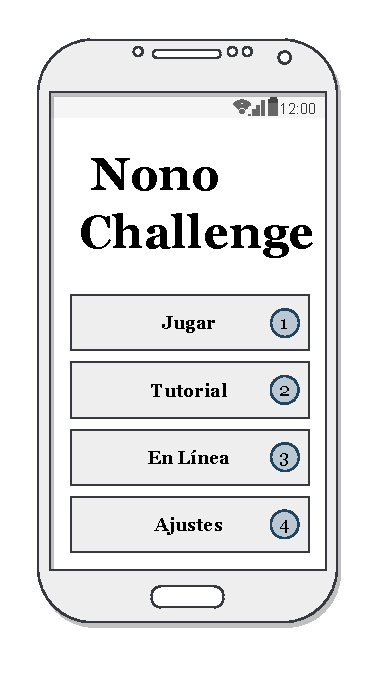
\includegraphics[width=\linewidth]{images/screen1.pdf}
    \end{subfigure}
    \begin{subfigure}[b]{0.38\linewidth}
      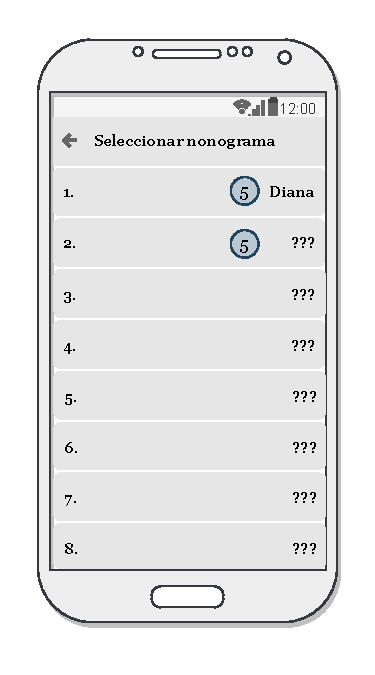
\includegraphics[width=\linewidth]{images/screen2.pdf}
    \end{subfigure}
    \caption{MockUps Pantalla de Inicio y Selector de niveles clásicos}
    \label{fig:design-1}
\end{figure}

La Pantalla de Inicio será la encargada de proveer al usuario el acceso de todos los casos
de uso y requisitos funcionales disponibles.

La pantalla de Selector de niveles clásicos mostrará todos los niveles disponibles predeterminados del sistema,
muchos de ellos extraídos de los libros \textit{Griddlers}, publicados por el noticiero británico 
\textit{Sunday Telegraph}.
A medida los niveles han sido superados se descubrirá el nombre de la figura que representa, Figura \ref{fig:design-1}.

\begin{figure}[H]
    \centering
    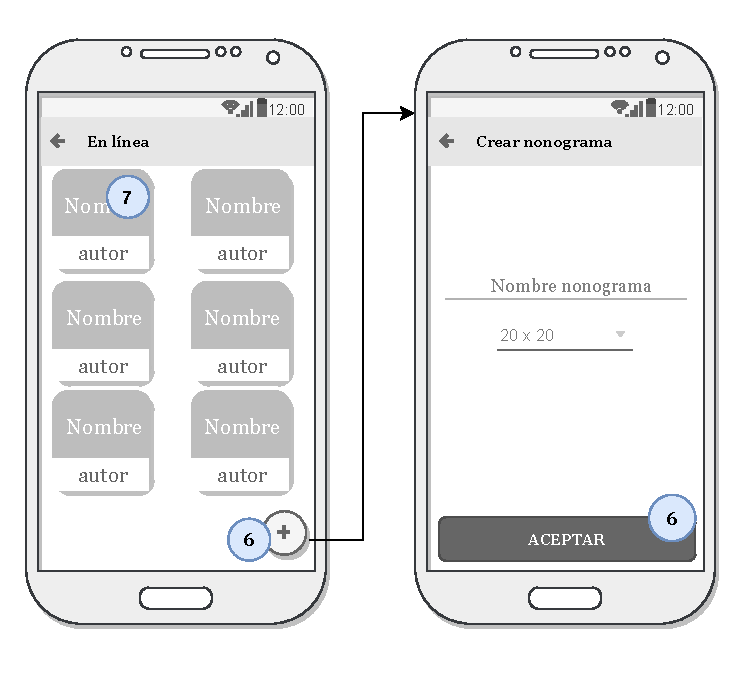
\includegraphics[scale=0.83]{images/screen3.pdf}
    \caption{MockUps Pantalla de niveles online y publicación de nonogramas}
    \label{fig:design-2}
\end{figure}

\begin{figure}[H]
  \centering
  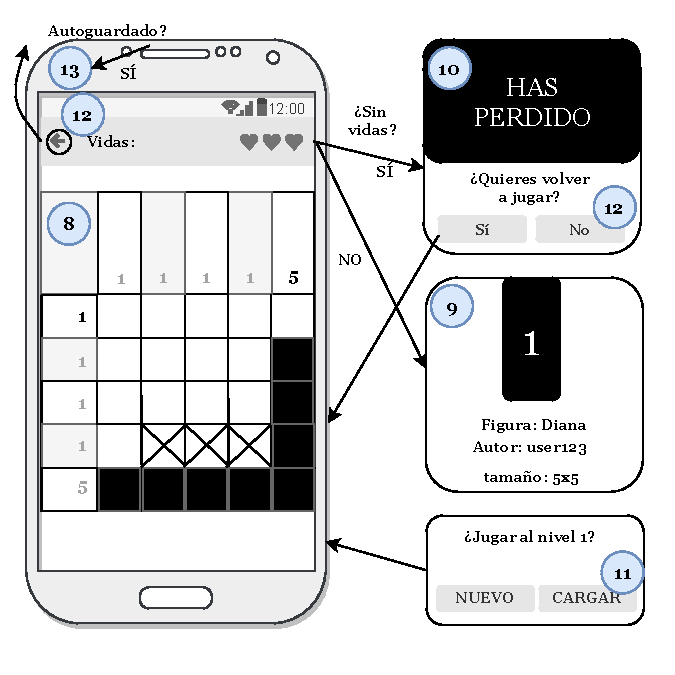
\includegraphics[scale=0.83]{images/screen4.pdf}
  \caption{MockUp Pantalla de resolución de nivel}
  \label{fig:design-3}
\end{figure}

En la Figura \ref{fig:design-3} se puede observar el diagrama de flujo de resolución
de nivel. 

La representación del rompecabezas es fiel al de los tradicionales:

\begin{itemize}
  \item[$\bullet$] Las celdas pintadas representan las celdas que se han seleccionado (con un clic) y
  resultan correctas
  \item[$\bullet$] Aquellas celdas con \textit{equis} son las marcadas  por el
  usuario (con doble clic sobre ella), asegurando que no son correctas.
  \item[$\bullet$] Los bloques de los extremos numerados, representan el número
  de celdas correctas de esa fila o columna, que se van difuminado a medida que se van
  resolviendo por el usuario.
\end{itemize}

El usuario puede abandonar el nivel en cualquier momento guardando su progreso si
la opción de autoguardado está activada. E 